\documentclass[10pt]{report}
\setcounter{tocdepth}{3}
\setcounter{secnumdepth}{3}
\usepackage[french]{babel}
\usepackage[a4paper, left=30mm,right=20mm,top=25mm,bottom=25mm]{geometry}
\usepackage{graphicx} % Required for inserting images
\usepackage[T1]{fontenc}
\usepackage{amstext}
\usepackage{float}
\usepackage{amsmath}
\usepackage{shorttoc}
\usepackage{hyperref}

\setlength{\parskip}{1ex plus 0.5ex minus 0.2ex}
\newcommand{\hsp}{\hspace{20pt}}
\newcommand{\HRule}{\rule{\linewidth}{0.5mm}}
\renewcommand\thesection{\arabic{section}}
\renewcommand{\contentsname}{Table des matières}


\begin{document}

\begin{titlepage}
  \begin{center}
    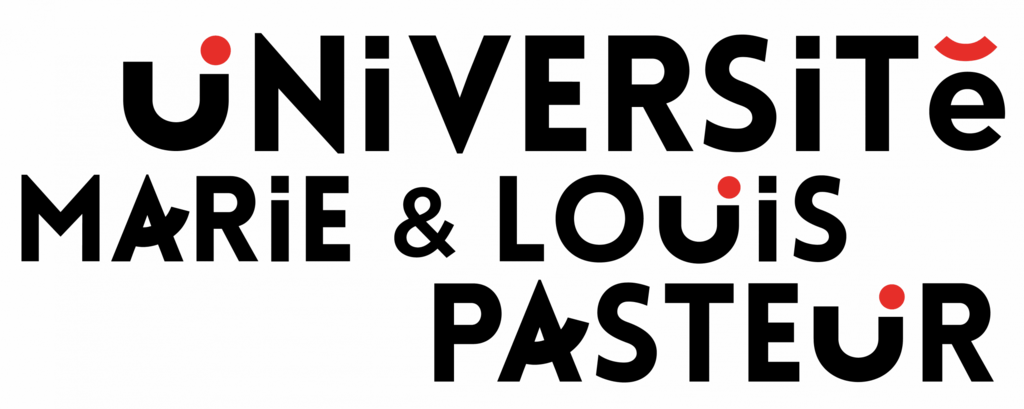
\includegraphics[height=25mm]{gfx/logo-UMLP} \\[1cm]
    

    {\LARGE\textsc{Université Marie et Louis PASTEUR}}\\[0.4cm]
    {\Large\textsc{UFR Sciences et Techniques}}\\[0.4cm]
    {\Large \textsc{L3 Informatique}}\\[1cm]
    

    \HRule \\[0.5cm]
    {\huge \bfseries Jeu de plate-formes avec génération procédurale}\\[0.4cm]
    \HRule \\[1cm]

    {\Large \textbf{Rapport de projet}}\\[1cm]

    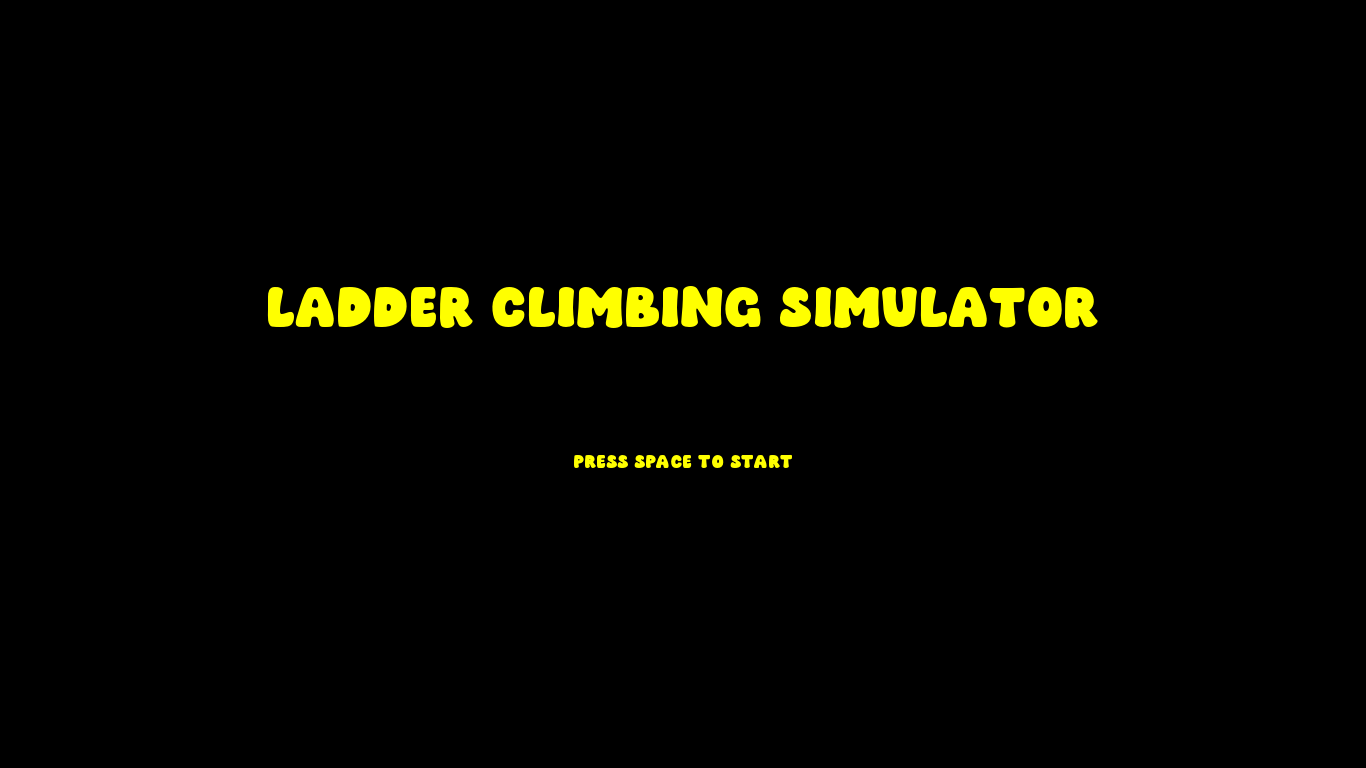
\includegraphics[width=0.7\textwidth]{images/illustration} \\[1.5cm]

    \parbox{0.45\textwidth}{\raggedright
      \textbf{Étudiants :} \\
      Kilian \textsc{Jelic}\\
      Laura\textsc{Jacqueson}\\
      Théo\textsc{Pariney}
    }
    \hfill
    \parbox{0.45\textwidth}{\raggedleft
      \textbf{Responsable :}\\
      Julien \textsc{Bernard}
    }
    \vfill

    {\large Mars 2025}

  \end{center}
\end{titlepage}

\normalsize
\pagenumbering{arabic}
\shorttableofcontents{Table des matières}{2}
\pagebreak
\listoffigures
\pagebreak

\section{Introduction}

Les jeux de plate-formes sont un genre qui repose sur le contrôle d'un personnage avec des mécaniques comme
les sauts et les obstacles, l’objectif étant généralement de rejoindre une sortie pour terminer le niveau.
L’ajout de la \textbf{génération procédurale} introduit une caractéristique supplémentaire :
plutôt que de concevoir chaque niveau à la main, un algorithme est chargé de créer les niveaux du jeu,
permettant ainsi une expérience unique à chaque partie.

Dans le cadre de notre projet semestriel en L3 Informatique à l'Université Marie et Louis Pasteur,
nous avons travaillé sur le développement d’un \textbf{jeu de plate-formes avec génération procédurale en C++}.

L'objectif principal de ce projet était de concevoir un jeu de plate-formes dont les niveaux seraient générés
de manière procédurale, offrant ainsi une rejouabilité infinie.
En parallèle, nous avons dû concevoir un jeu intégrant plusieurs mécaniques de jeu, incluant des déplacements,
des sauts, un dash, ainsi qu’un objectif centré sur la récolte d’objets, tout en assurant la gestion des collisions et la physique du jeu.

Dans ce rapport, nous commencerons par une présentation générale du jeu, en exposant les objectifs du joueur et
les scènes du jeu.
Ensuite, nous détaillerons la conception des blocs et entités qui composent le monde et leur gestion dynamique.
Par la suite, nous aborderons la génération procédurale, en expliquant la méthode utilisée ainsi que les détails
d'implémentation.
Nous discuterons ensuite des contrôles du personnage et des différentes mécaniques de jeu, telles que le saut,
le dash, etc.
La partie suivante sera consacrée à la physique, notamment la gestion des collisions et des propriétés physiques
comme la résistance de l'air.
Enfin, nous reviendrons sur l’organisation du travail, la répartition des tâches et les outils utilisés pour
mener à bien ce projet.
Le rapport se conclura par un bilan du projet et les améliorations possibles.

\pagebreak



\section{Présentation du jeu}
\subsection{Présentation générale}

Ce projet consiste à développer un \textbf{jeu de plate-forme en 2D} intégrant un système de \textbf{génération procédurale} de niveau.
L’objectif est d’offrir une expérience où chaque partie est unique : au lieu d’avoir des niveaux prédéfinis,
ceux-ci sont générés aléatoirement à chaque nouvelle partie.
Contrairement aux jeux de plate-forme classiques où l'on peut apprendre les niveaux par cœur, ici, aucun parcours ne
peut être rejoué à l’identique.
Cette approche permet non seulement une rejouabilité infinie, mais aussi un défi durable, obligeant le joueur
à s’adapter à chaque nouvelle configuration de niveau.

Le joueur incarne un petit robot, dont la mission principale est de récolter un maximum d’écrous
avant d’atteindre la sortie du niveau.
Ces écrous sont disposés aléatoirement dans l’environnement, incitant le joueur à explorer avant de pouvoir
terminer la partie.

\begin{figure}[H]
  \centering
  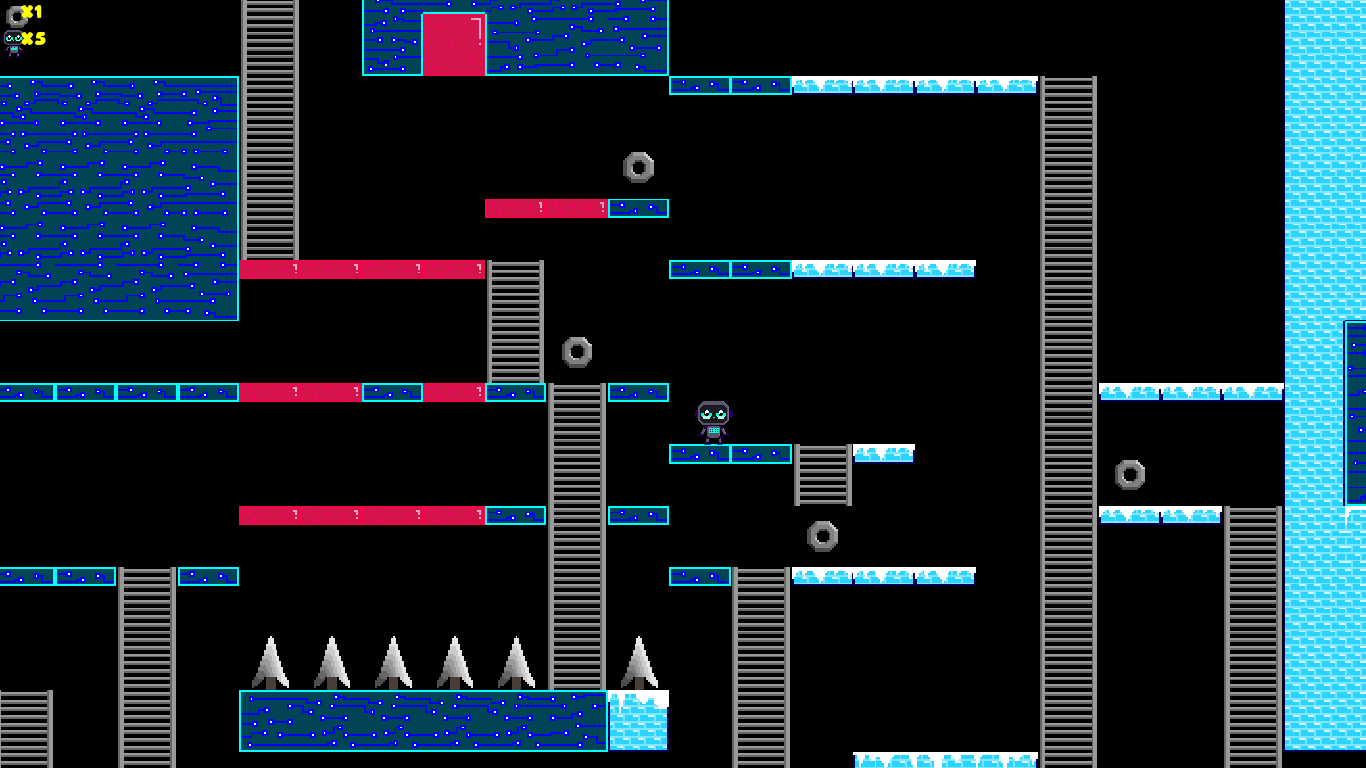
\includegraphics[width=0.5\textwidth]{images/world_example}
  \caption{Exemple de monde}
\end{figure}


Pour naviguer dans le monde, le joueur dispose de plusieurs mécaniques lui permettant de se déplacer librement et
d’interagir avec son environnement :
\begin{itemize}
  \item \textbf{déplacement} : le personnage peut se déplacer latéralement, à gauche et à droite,
  pour parcourir le niveau.
  \item \textbf{saut} : le personnage peut sauter pour franchir des obstacles ou atteindre des plateformes
  situées en hauteur.
  \item \textbf{double saut} : après un premier saut, lorsqu'il est encore en l’air, le personnage peut effectuer
  un second saut lui permettant d’atteindre des zones plus élevées.
  \item \textbf{dash} : le personnage dispose également d’un dash, une impulsion rapide dans une direction
  (gauche ou droite), utile pour traverser de grands espaces vides ou esquiver des obstacles.\\
\end{itemize}

Ces mécaniques offrent une grande liberté d'action, permettant aux joueurs d’adopter différentes stratégies.
Certains préfèreront une approche prudente, en évitant à tout prix de mourir, tandis que d’autres tenteront de terminer simplement le niveau sans se soucier de la mort.


Comme mentionné précédemment, tous les niveaux sont générés de manière procédurale, cela signifie qu'à chaque
lancement de partie c'est un algorithme qui se charge de créer un environnement en plaçant des blocs, plateformes,
échelles, écrous, piques et une sortie.
Cette méthode permet de générer de manière presque infinie des mondes différents.

Ces différent niveaux sont composés de salles générées de manière 
contiguës, et les salles sont reliées entre elles par des échelles et des
plateformes, de façon à ce que chaque niveau soit possible, en partant du
début jusqu'à la fin.
Des blocs et plateformes de glace et de slime sont
également générés, et le joueur doit donc faire attention aux changements 
que cela implique sur ses déplacements.


\subsection{Les objectifs du joueur}

Dans ce jeu de plate-forme, le joueur incarne un petit robot dont l’objectif principal est de récupérer des écrous
dispersés dans l’environnement avant d’atteindre la sortie.


\subsubsection{Les écrous}

Les écrous sont des objets collectables répartis à plusieurs endroits du niveau.
Ils constituent un élément central du jeu, car ils encouragent le joueur à explorer le monde plutôt que de se
précipiter vers la sortie.

\begin{figure}[H]
  \centering
  
\includegraphics[width=0.3\textwidth]{images/nut}
  \caption{Ecrou}
\end{figure}

Comme tous les autres éléments du monde, les écrous sont placés aléatoirement à chaque génération de niveau.
Leur nombre n’est pas fixe, ce qui signifie que chaque partie offre une répartition différente des écrous,
renforçant ainsi la rejouabilité.
Le joueur doit donc parcourir l’environnement avec attention pour être sûr de ne pas en oublier.

Toutefois, la collecte des écrous n’est pas obligatoire pour terminer un niveau.
Le joueur peut choisir de se concentrer sur la recherche de la sortie ou, au contraire, tenter de récupérer
un maximum d’écrous pour améliorer son score, affiché dans le coin supérieur gauche de l’écran.


\subsubsection{La sortie}

La sortie représente l'objectif final d'une partie.
Une fois que le joueur l'a trouvée, il peut choisir de l’atteindre immédiatement pour terminer la partie ou bien
continuer à explorer afin de collecter davantage d’écrous et améliorer son score.
Ce choix introduit un élément de stratégie, puisque le joueur doit évaluer s’il préfère sécuriser sa progression
ou prendre des risques pour maximiser ses points.

\begin{figure}[H]
  \centering
  
\includegraphics[width=0.2\textwidth]{images/exit}
  \caption{Sortie}
\end{figure}


Comme pour les écrous, la sortie est placée aléatoirement dans le niveau, ce qui signifie que le joueur ne sait
jamais à l’avance où elle se trouve.
Il est donc obligé d’explorer activement l’environnement pour la localiser.

Le fait que la sortie soit générée aléatoirement renforce la diversité des parties.
Chaque session de jeu demande au joueur de s’adapter aux conditions spécifiques du niveau généré, ce qui augmente
le défi et évite toute monotonie.
Trouver la sortie peut parfois être simple, mais dans d’autres cas, elle pourra être bien cachée ou difficile d’accès,
obligeant le joueur à parcourir l’intégralité du niveau.

Enfin, atteindre la sortie ne signifie pas nécessairement que le joueur a maximisé son score, mais cela valide
sa progression et lui permet de lancer une nouvelle partie avec un niveau entièrement différent.

\subsection{Les scènes}

Le jeu est organisé en scènes, pour permettre des boucles de jeu différentes.
Les scènes sont des objects à part entière contenant l'ensemble des entités, textes, et actions pouvant être réalisées sur celle-ci.
Celles-ci sont elles-même stockées dans l'object \emph{PlatformerManager}, un gestionnaire de scènes ayant pour rôle de changer la scène active.
Le jeu est composé des scènes :\\
\begin{itemize}
  \item \textbf{Menu} : La scène affichée lors du lancement du jeu.
  Elle contient seulement un texte expliquant comment lancer le jeu, et le titre du jeu.
  Elle permet de lancer le jeu avec la touche \emph{espace}, et de quitter le jeu avec la touche \emph{echap}.
  \item \textbf{GameScene} : La scène principale du jeu.
  Elle contient tous les objets du monde et le personnage.
  La plupart des actions de la scène servent à déplacer le personnage.
  Il est possible d'afficher un menu de pause depuis cette scène à l'aide des touches \emph{P} et \emph{echap}.
  \item \textbf{Pause} : Menu affiché quand la \emph{GameScene} est en pause.
  Elle contient seulement un texte expliquant le menu de pause.
  Elle laisse la scène principale en arrière plan, en pause.
  Il est possible de la quitter avec les touches \emph{P} et \emph{echap}.
  \item \textbf{EndScene} : La scène de fin de jeu.
  Elle affiche le résultat de la partie (si le joueur est mort ou non et son score), et permet de retourner au menu principal avec la touche \emph{espace}.
\end{itemize}

\section{Les blocks et entités du monde}
\subsection{La définition dynamique des blocs}
L'ensemble des éléments qui composent le monde (blocs, écrous, sortie\ldots) sont définis de manière dynamique dans le fichier XML tiles.xml.\\
Nous avons fait le choix d'utiliser XML car il s'agit d'un type de fichier encore très utilisé, mais absent de notre formation.\\
Ce fichier permet de donner les éléments pouvant être utilisés par le jeu et la génération sans avoir à ré-écrire d'importantes parties du code à chaque ajout de fonctionnalité dans le monde.\\
La racine de l'arborescence XML donne le chemin vers les textures des éléments.\\
Au sein du fichier, un élément est donné par un bloc, correspondant à son type principal, et donnant le comportement général de l'élément.
Les autres caractéristiques donnant le comportement des éléments sont :\\
\begin{itemize}
  \item \textbf{type}: Le sous-type de bloc correspond au nom de bloc, permettant de lui définir un comportement unique, en plus de son type principal.
  Par exemple, un bloc de type plateforme peut être une plateforme de glace ou une plateforme de slime.
  Ces deux types de plateformes auront un attribut ``type'' différent.
  \item \textbf{texture}: Le chemin relatif de la texture de l'élément à partir du chemin donné dans la racine.
  \item \textbf{scale}: Le paramètre de mise à l'échelle de la texture.
  \item \textbf{staticFriction} et \textbf{dynamicFriction} : Respectivement, les coefficients de friction statiques et dynamiques de l'élement (cf. \ref{physique:friction})
  \item \textbf{restitution} : Le coefficient de restitution de l'élément (cf. \ref{physique:collisions})
  \item \textbf{collidable}: Définit si le bloc est solide et est pris en compte dans les collision ou pas.
  \item \textbf{direction}: Indique si le bloc est directionnel, et donne sa direction (cf. \ref{physique:direction})
  \item \textbf{connected} : Indique si la texture de l'élément doit être connectée aux textures des éléments du même sous-type.
  \item \textbf{hitboxHeight, hitboxWidth, hitboxOffsetX, hitboxOffsetY}: Paramètres de taille et de positionnement de la hitbox du bloc.
  de la boîte de collision.
\end{itemize}

Ce fichier XML est lu par une classe \emph{BlockTypes} qui va stocker les types de blocs sous forme de structures \emph{BlockType} afin qu'ils puissent être utilisés par les autres éléments du jeu.
  
\subsection{Le stockage des blocs}

Les blocs sont stockés et gérés par un objet \emph{BlockManager}.

Cet objet permet de stocker les blocs du monde dans un tableau associatif, en associant une position dans le plan à un nom de bloc.
Nous pouvons donc par la suite, à partir du type de bloc, lire ses propriétés à l'aide d'une méthode statique de la classe \emph{BlockTypes}.

\subsection{La connectivité des textures}

Pour un meilleur aspect esthétique, les textures des blocs de même sous-type peuvent se connecter entre elles.

Pour les éléments de jeu classiques, les textures sont des images simples qui correspondent à la texture du bloc.
Pour les blocs possédant la propriété ``connected'', la texture est stockée sous la forme d'une spritesheet,
donnant les 16 textures possibles pour chaque bloc, pour que la connection se fasse, en fonctions des blocs qui l'entourent.

\begin{figure}[H]
  \centering
  
\includegraphics[width=1.0\textwidth]{images/tile_jelly}
  \caption{Spritesheet du bloc de gelée, possédant la propriété connected}
  \label{fig:tile_jelly}
\end{figure}

Pour cela, le \emph{BlockManager} associe à une position, en plus du type de bloc s'y trouvant, un indice sous la
forme d'un entier non signé indiquant quelle partie de la spritesheet appliquer.
Lors de la création du \emph{BlockManager}, cet entier est positionné à 0, et les blocs ont leur texture ``par défaut'', sans connections.
Une fois le monde généré, et l'ensemble des blocs du monde stockés dans le \emph{BlockManager}, celui-ci recalcule l'indice de texture des blocs en fonction des blocs du même type qui l'entourent :

\begin{figure}[H]
  \centering
  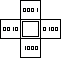
\includegraphics[width=0.5\textwidth]{images/connected_textures_offset_computing}
  \caption{Calcul de la connectivité des textures.}
  Le bloc central est celui dont on veut déterminer la texture.\\
  L'indice de la texture du bloc central est donné par la somme des nombres indiqués sur la figure des blocs adjacents du même type.
  \label{fig:connected_textures_computing}
\end{figure}

Un bit est donnée à chaque position de bloc pouvant entourer le bloc donc on veut déterminer la texture:
\begin{itemize}
  \item \textbf{0001} Pour le bloc au dessus
  \item \textbf{0010} Pour le bloc à gauche
  \item \textbf{0100} Pour le bloc à droite
  \item \textbf{1000} Pour le bloc au dessous
\end{itemize}
On fait la somme des nombres associés aux blocs adjacents du même sous-type que le bloc, ce qui nous donne l'indice de la texture à appliquer.

\begin{figure}[H]
  \centering
  
\includegraphics[height=0.2\textwidth]{images/connectedTiles}
  \caption{Groupe de 4 blocs de gelée dont les textures se connectent entre elles}
  \label{fig:connected_tiles}
\end{figure}

\subsection{Le monde}

L'objet \emph{World} est composé de plusieurs choses dont: un générateur de monde, un conteneur d'entités,
un \emph{BlockManager}, un joueur, un point d'apparition de joueur, et enfin d'une limite inférieure au monde.

Cet objet permet de centraliser tous les objets qui doivent être mis à jour à chaque frame de jeu, afin de
les mettre à jour plus facilement.

La limite inférieure de monde sert à s'assurer que même dans le cas où le joueur trouverait un moyen de sortir de la
zone de jeu et tomberait dans le vide, qu'il soit téléporté à son point d'apparition.
Cette limite inférieure est calculée à partir de la salle la plus basse qui ait été générée par le générateur de monde.

\section{La génération procédurale}
\subsection{Aléatoire et graine de génération}

À des fins de débuggage, la possibilité de pouvoir générer le même monde plusieurs fois est importante.
Pour cela, les niveaux sont générés à l'aide d'un générateur de nombres pseudo-aléatoire.
Ce générateur peut utiliser un entier codé sur 64 bits, et générera la même séquence de nombres
aléatoires tant que la même graine est utilisée. 

Nous avons donc implémenté deux moyens de générer les mondes: avec ou sans graine.
Si une graine est donnée au générateur, alors cette graine sera utilisée lors de la création du niveau.
Sinon, une graine aléatoire est choisie, et est affichée dans la console.
Cela permet, en cas de problème, de facilement noter et partager une graine, permettant de reproduire
le problème plus facilement.

\subsection{Étapes de génération}
\subsubsection{Génération des salles}

Les salles sont générées de manière à ce qu'elles soient connectées entre
elles, sans jamais se chevaucher.
Pour cela, l'algorithme suivant est appliqué:

\begin{itemize}
  \item Générer une salle de départ.
  \item Tant que le nombre de salles voulu n'est pas atteint:
  \begin{itemize}
    \item Choisir aléatoirement la taille de la salle.
    \item Choisir une direction (haut, bas, gauche ou droite)
    \item Créer une nouvelle salle, placée à côté de la salle précédente,
    aléatoirement le long du mur correspondant à la direction choisie.
    \item Si la salle chevauche une autre salle, la regénérer.
    \item Si, au bout d'un certain nombre d'essais, la salle n'a pas réussi
    à se générer, réessayer en changeant la taille de la salle.
    \item Si la salle n'arrive toujours pas à se générer, supprimer la
    salle ainsi que la salle précédente, et regénérer la salle précédente.
  \end{itemize}
\end{itemize}

Certains cas spéciaux se présentent avec cet algorithme:
\begin{itemize}
  \item \textbf{La salle de départ}: La salle de départ, étant la première
  salle, ne peut pas se générer à la suite d'une autre salle.
  Elle se génère donc simplement aux coordonnées (0, 0)
  \item \textbf{Retour en arrière}: Dans certains cas, une salle peut se 
  retrouver encerclée par d'autre salles.
  Dans ce cas, aucune salle ne pourra se générer par la suite.
  Afin d'éviter ces situations, l'algorithme décide, si une salle n'arrive pas à se générer, de réessayer
  d'abord avec une salle de différente taille, car une salle plus petite
  peut éventuellement réussir à se générer.
  Mais, au bout d'un certain nombre d'essais, l'algorithme décide de retourner en arrière.
  Dans ce cas, la salle précédente est supprimée, et, en prenant un autre chemin,
  le générateur réussira à générer l'ensemble des salles.
  \item \textbf{Taille minimale d'entrée}: La génération de plateformes et 
  de pièges pourrait rendre l'entrée dans une salle impossible dans des cas
  où l'entrée d'une salle serait trop petite.
  Afin d'éviter cela, lorsqu'elles se placent le long d'un mur, les coordonnées aléatoires ont
  été restreintes afin que l'entrée vers la salle suivante aie toujours
  une taille minimale.
  Cette taille a été définie à 2 blocs.
  Dans la figure~\ref{fig:room_placement}, on peut voir que peu importe où se génère la
  salle, l'entrée de la salle verte vers la salle bleue aura toujours une
  taille d'au moins 2 blocs.
\end{itemize}

\begin{figure}[H]
  \centering
  
\includegraphics[width=0.5\textwidth]{images/room_placement}
  \caption{Un exemple de placement de salle.}
  Une salle est représentée en vert.\\ 
  Si la direction haut est choisie, une salle de taille 3x3 peut\\
  se générer n'importe où dans la zone bleue.
  \label{fig:room_placement}
\end{figure}

Les salles étant une donnée réutilisée fréquemment par le générateur,
elles sont stockées en tant que liste de vecteurs contenant une position
x et y, ainsi que la taille de la salle (voir figure~\ref{fig:room_data}).

\begin{figure}[H]
  \centering
  
\includegraphics[width=0.5\textwidth]{images/room_storage}
  \caption{Une représentation du stockage d'une salle, 
  en tant que coordonnée et taille de salle}
  \label{fig:room_data}
\end{figure}

\subsubsection{Génération des murs}

Une fois les salles générées, les murs sont placés.
Pour cela, le niveau est rempli avec des blocs, de manière à recouvrir complètement toutes
les salles, plus une marge afin de marquer la bordure du niveau. 
Les coordonnées de remplissage correspondent simplement aux coordonnées
minimum et maximum correspondant à des salles.
Ensuite, des blocs sont retirés de manière à creuser les salles.

\begin{figure}[H]
  \centering
  
\includegraphics[width=0.5\textwidth]{images/filling_the_world}
  \caption{Deux salles, après que les murs soient générés}
  \label{fig:filling_world}
\end{figure}

\subsubsection{Génération du chemin}

La prochaine étape de la génération est de générer un chemin, que le 
joueur pourra suivre.
Cela permet de s'assurer qu'il existe toujours au
moins un chemin possible afin de terminer le niveau, et que tous les 
niveaux soient bien possibles.

Le chemin est une suite de coordonnées.
Un point est donc choisi aléatoirement dans chaque salle.

Une fois le chemin généré, afin que le joueur puisse l'emprunter, il
faut le relier avec des plateformes et des échelles.
Pour cela, nous utilisons un algorithme dont le but est de tracer des
lignes droites, en zig-zag:

\begin{itemize}
  \item Choisir une direction (horizontale ou verticale)
  \item Tant que possible, avancer dans la direction choisie vers le
  point de destination
  \item Si le point de destination est atteint dans la direction choisie
  ou que l'on ne peut plus avancer, changer de direction et continuer
  \item S'arrêter une fois que le point est atteint, ou si aucun chemin 
  n'est trouvé
\end{itemize}

Une fois le chemin calculé, les sections horizontales du chemin seront
remplacées par des plateformes, et les sections verticales correspondront
à des échelles.

Afin d'introduire plus de variété, le chemin est calculé deux fois:
En commençant par la direction horizontale (plateforme), et en commençant
par la direction verticale (échelle).
Si le chemin a pu être tracé dans les deux directions, une des deux directions est choisie aléatoirement.
Si seule un des deux chemins a pu être tracé entièrement, alors celui-ci est choisi.

\begin{figure}[H]
  \centering
  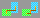
\includegraphics[width=0.5\textwidth]{images/two_ways_to_connect}
  \caption{Un chemin composé de deux points, et les deux manières de
  les connecter}
  (En commençant par une échelle à gauche, et par une plateforme à droite)\\
  On peut remarquer que le chemin s'arrête avant de toucher le plafond, 
  afin que le joueur puisse marcher sur la plateforme.
  \label{fig:two_ways_to_connect}
\end{figure}

Encore une fois, certains cas particuliers apparaissent:
\begin{itemize}
  \item \textbf{Le dernier point}: Le dernier point du chemin correspondra à la sortie.
  Il est donc placé de manière particulière, en utilisant le
  même algorithme que pour touver un point de départ qui soit sécurisé (voir section~\ref{subsubsec:spawn_point}).
  \item \textbf{Prise en compte du plafond}: Une fois les plateformes
  générées, il est important que le joueur puisse marcher sur les plateformes.
  Ainsi, si en générant une échelle ou une plateforme, si
  l'algorithme rencontre un espace où le plafond ne permet pas de marcher
  sur la plateforme, cet espace est considéré comme un mur, causant un
  changement de direction.
  \item \textbf{Connections entre échelle et plateforme}: Afin de connecter
  correctement une plateforme et une échelle, certains cas particuliers
  sont pris en compte, particulièrement lorsqu'il s'agit de choisir le bloc
  correspondant à un coin lors d'un virage.
  Pour cela, si une échelle vient du bas de la plateforme, alors le bloc du coin sera une échelle.
  Sinon, le bloc sera une plateforme.
  Ces choix sont visibles sur la figure~\ref{fig:two_ways_to_connect}.
\end{itemize}

\subsubsection{Placement de la sortie}

La sortie est placée à la position du dernier point du chemin, selon
les conditions indiquées ci-dessus.

\subsubsection{Fausses plateformes et échelles}

Un jeu dont le chemin serait tout tracé ne serait pas amusant.
Pour cette raison, nous essayons de brouiller les pistes en noyant le
véritable chemin au milieu de fausses plateformes et échelles.
Ces plateformes sont générées aléatoirement dans chaque salle.
Chaque plateforme est placée en commençant sur le mur gauche ou droit,
et est placée bloc par bloc vers l'intérieur de la salle jusqu'à ce
que la plateforme croise un bloc sur son chemin ou
que la plateforme atteigne une taille choisie aléatoirement.
Par la suite,des échelles sont générées le long de la plateforme,
s'étendant vers le bas suivant le même principe que les plateformes.

\begin{figure}[H]
  \centering
  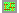
\includegraphics[width=0.5\textwidth]{images/fake_platforms}
  \caption{Un exemple de génération de fausse plateformes}
  \label{fig:fake_platforms}
\end{figure}

\subsubsection{Placement des blocs spéciaux}

Afin de pimenter la traversée du niveau par le joueur, de la glace et du 
slime sont placés dans ce niveau.
Cela transforme les blocs et les plateformes en leur version de glace ou de slime.
Le choix de la variante de bloc est déterminé par un bruit de Perlin, appliqué sur chaque bloc
composant le niveau.
Cela fait que la plupart du niveau sera normal, mais que certaines zones seront plus glacées,
et d'autres zones seront plutôt recouvertes de slime,
sans qu'une transition trop brusque entre les zones ne soit visible.

\subsubsection{Placement des pièges}

Des dangers et pièges sont ensuite rajoutés au niveau, afin que le joueur ne puisse pas se déplacer librement sans
faire attention, et augmentant la difficulté du jeu.
Pour cela, des pics sont rajoutés au niveau.
Si le joueur touche un de ces pics, il sera instantanément ramené au début du niveau, et perdra une vie.
Les pics sont rajoutés de deux manières.
\begin{itemize}
  \item Premièrement, chaque salle a 30\% de chance d'être rendue dangereuse.
  Cela implique que le sol de la salle sera recouvert de pics.
  \item Ensuite, d'autres petits pièges, plus rares et moins importants, sont rajoutés dans toutes les salles.
  Actuellement, seul un type de piège est implémenté: si une ligne de blocs de glace est détectée au sol, alors
  un pic est placé au bout de cette ligne.
  Cela fait que si le joueur marche sur ce sol de glace, il prend alors le risque de glisser, et d'être tué par le
  pic se trouvant au bout.
\end{itemize}

La dernière salle est épargnée par ces mécaniques.
De cette manière, aucun pic ne se générera dans la salle contenant la sortie, évitant des situations où la sortie
difficile d'accès car se trouvant au milieu de pics.

  \begin{figure}[H]
  \centering
  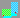
\includegraphics[width=0.5\textwidth]{images/ice_spike_trap}
  \caption{Un exemple de génération de pics dans des salles.}
  Seule la salle bleue a été sélectionnée comme étant dangereuse.\\
  Le pic de la salle verte est placé au bout d'une ligne de blocs de glace.
  \label{fig:spike_placement}
\end{figure}

\subsubsection{Placement du point d'apparition}
\label{subsubsec:spawn_point}

Le joueur ne peut pas commencer le niveau à n'importe quelle position.
Il faut s'assurer que le joueur ne commence pas le niveau dans un endroit dangereux, ou flottant dans les airs.
Pour cela, étant donné une salle, l'algorithme suivant cherche un point d'apparition valide dans la salle:

\begin{itemize}
  \item Vérifier le bloc situé au sol, au milieu de la salle.
  \item Si ce bloc est vide, et que le bloc situé juste en dessous est un bloc solide, alors il s'agit d'un
  point d'apparition valide.
  \item Sinon, on vérifie les blocs situés sur la même ligne, à gauche est à droite, en partant du centre jusqu'au
  bord de la salle.
  \item Si aucun point d'apparition n'est trouvé sur cette ligne, chercher sur la ligne située un bloc plus haut.
\end{itemize}

Si, pour une raison quelconque, aucun point d'apparition n'est trouvé, alors un point d'apparition valide est
cherché dans les salles suivantes.

\begin{figure}[H]
  \centering
  
\includegraphics[width=0.5\textwidth]{images/valid_spawn_locations}
  \caption{Un exemple des points d'apparition valides dans un niveau.}
  Le bloc situé le plus au centre, en bas de la salle de départ sera le point d'apparition choisi.
  \label{fig:spawn_points}
\end{figure}

\subsection{Monde de test}

Afin de tester des fonctionnalités du jeu comme les collisions, les 
échelles ou autres, un monde de test a été ajouté, sous la forme d'un 
générateur de monde.
Dans le code, nous pouvons changer le générateur de
niveau en notre générateur de monde de test, et le monde généré sera alors
un monde simple, contenant une plateforme et autres fonctionnalités que
nous voulons tester (voir figure~\ref{fig:test_world}).

\begin{figure}[H]
  \centering
  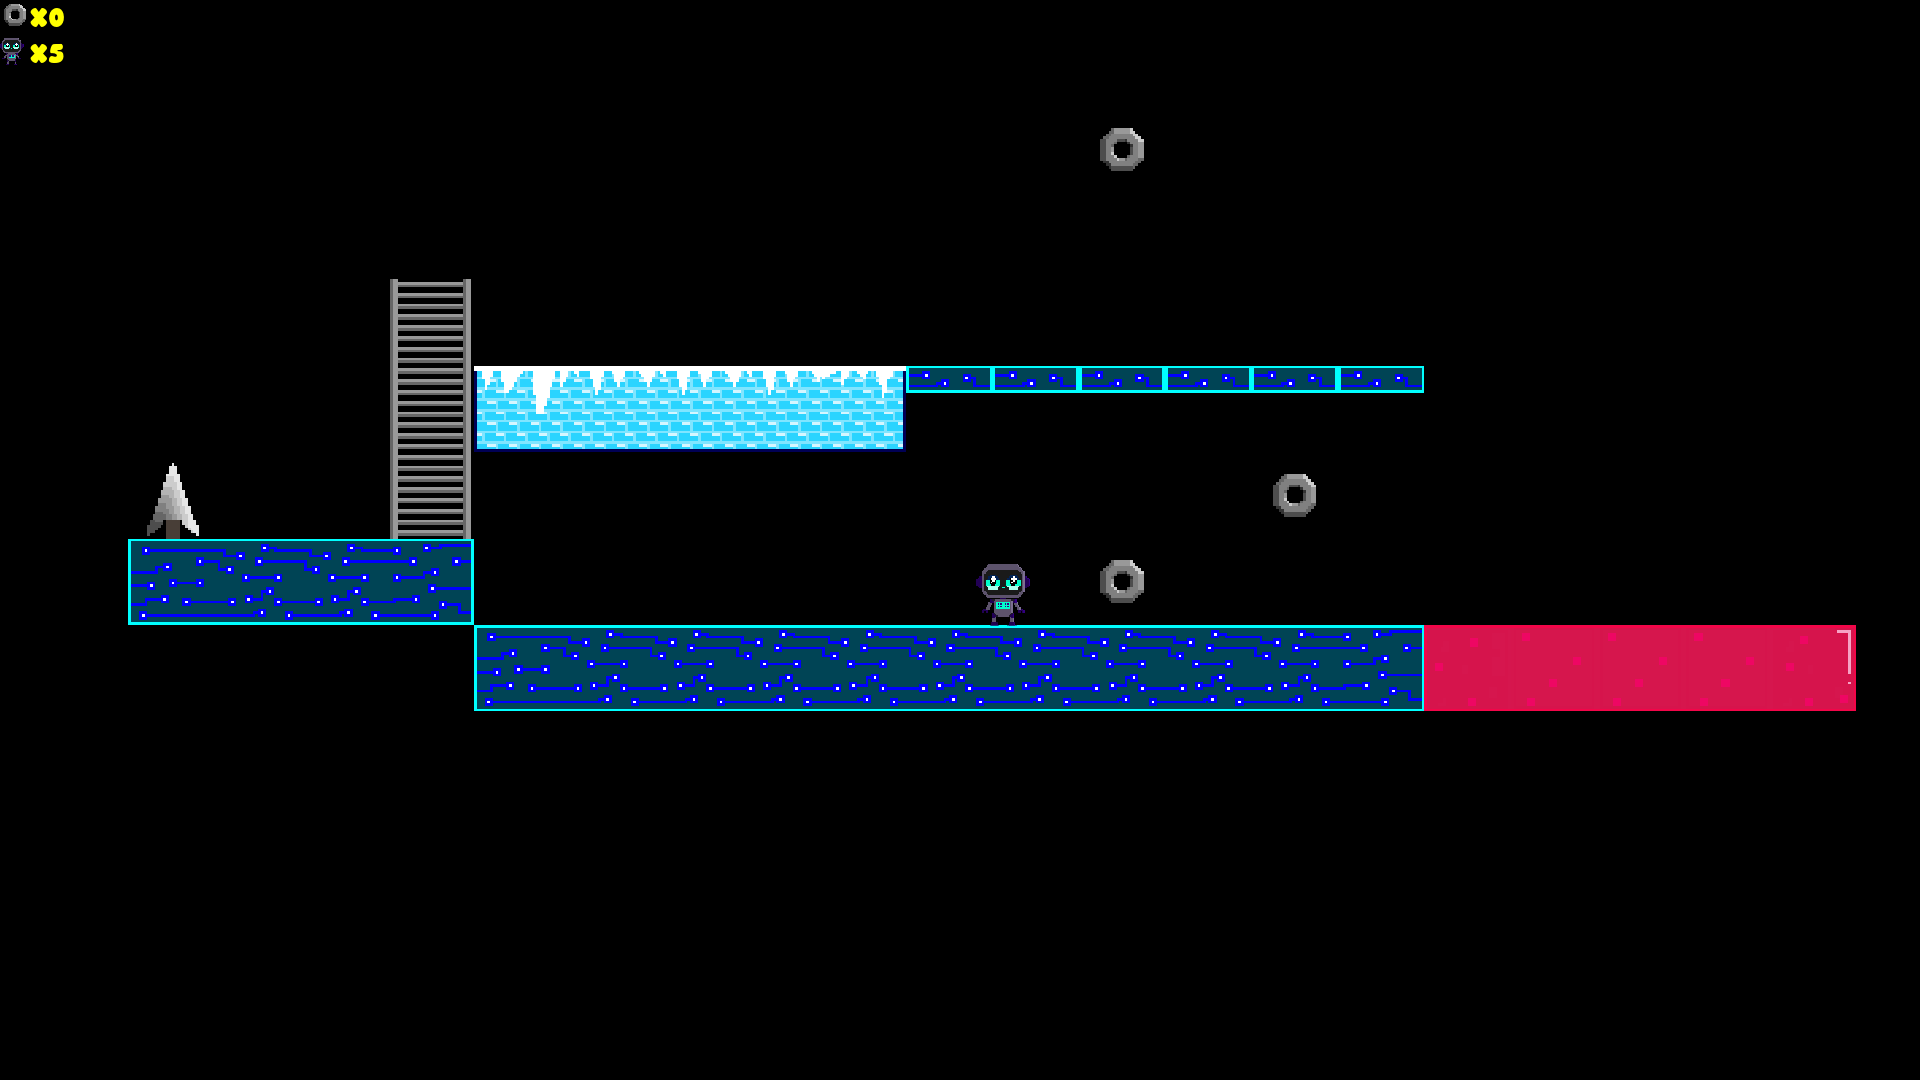
\includegraphics[width=\textwidth]{images/test_world}
  \caption{Une capture d'écran du monde de test}
  \label{fig:test_world}
\end{figure}

\section{Le personnage}
Le joueur incarne un petit robot doté de différentes possibilités de déplacement, lui permettant d'évoluer dans le niveau.


\begin{figure}[H]
  \centering
  
\includegraphics[width=0.3\textwidth]{images/character_placeholder}
  \caption{Le personnage}
\end{figure}

\subsection{Les contrôles de base}
Le personnage se déplace principalement à gauche et à droite. Ces déplacements sont possibles grâce aux flèches directionnelles (droite $\rightarrow$ ou gauche $\leftarrow$) ou bien les touches \emph{"Q"} et \emph{"D"}.\\
Ce fonctionnement repose sur plusieurs mécaniques assurant un déplacement horizontal fluide :

\begin{itemize}
  \item \textbf{Déplacement droite/gauche} : lorsque le joueur appuie sur les touches de déplacement, une constante est ajoutée à l'axe X du personnage lui permettant de gagner de la vitesse.
  \item \textbf{Priorité} : si les 2 touches sont pressées en même temps, la priorité de déplacement est donnée à la droite.
  \item \textbf{Effet de la glace} : Lorsque le personnage se trouve sur un bloc ou une plateforme de glace, il ne s'arrête pas immédiatement après le relâchement de la touche. De plus, comme la glace n'a pas de friction, le personnage est affecté par cette absence de friction et va donc plus vite pendant son déplacement.
\end{itemize}

Ces déplacements sont controlés via des actions continues, c'est-à-dire que tant que la touche en enfoncée le joueur continue de se déplacer. 


\subsection{Le saut}
Le personnage peut sauter en appuyant sur la touche \emph{Espace} du clavier. Les sauts sont essentiels pour un jeu de plateforme, car sans eux, le personnage ne pourrait pas franchir d'obstacles ni atteindre les plateformes en hauteur. 

Lors de l'appui de la touche \emph{Espace}, le personnage monte, et la hauteur maximale atteinte, il redescend progressivement. \\
Sur le plan technique le saut repose sur les principes suivants : 

\begin{itemize}
  \item \textbf{Impulsion initiale} : au moment du saut, une constante est ajouté sur l'axe Y du personnage, lui permettant de quitter le sol.
  \item \textbf{Influence de la gravité} : une fois arrivé à son point maximum le personnage redescend doucement sous l'effet de la gravité. 
  \item \textbf{Influence de la résistance de l'air} : lors de la montée ainsi que de la descente, le personnage est ralentit sous l'influence de la résistance de l'air, ce qui permet de ne pas avoir d'accélération brutale. 
  \item \textbf{Condition d'activation du saut} : un saut ne peut être initié que si le joueur est en contact avec le sol (plateformes ou blocs), ce qui signifie que s'il est sur une échelle le saut est impossible. 
\end{itemize}

En plus du saut classique, le personnage à la possibilité d'effectuer un \textbf{double saut}. Cette mécanique permet au joueur, une fois que le robot est en l'air, de réappuyer sur \emph{Espace} pour lui donner une nouvelle impulsion pour atteindre des endroits plus en hauteur. 

En plus des principes du saut simple, le double saut repose également sur ces principes :

\begin{itemize}
  \item \textbf{Déclenchement} : le joueur peut appuyer sur la touche du saut avant que le personnage n'atterrisse sur le sol, ce qui applique de nouveau une impulsion vers le haut.
  \item \textbf{Limitation} : le double saut ne peut être utilisé qu'une fois par saut simple. Pour réinitialiser cette capacité le personnage doit retoucher le sol.
\end{itemize}


Nous avions initialement prévu d'intégrer un saut modulable au jeu. Cette mécanique permettait au joueur de contrôler la hauteur du saut du personnage en fonction de la durée d'appui sur la touche. Plus la touche aurait été maintenue, plus le robot serait allé haut, avec un plafond maximum.
Cependant, nous avons fait le choix d'abandonner cette mécanique car elle compliquait trop les commandes au clavier rendant les sauts moins intuitifs et plus difficiles à maîtriser. 

\subsection{Le dash}
Le dash est une mécanique permettant au personnage d'effectuer une accélération horizontale afin d'atteindre un point éloigné plus rapidement. Il peut aussi être combiné au saut pour donner plus de choix de mobilité au joueur.

Dès le début de l'implémentation de cette mécanique, nous avons rencontré des difficultés pour le choix de la commande déclenchant le dash. Au départ, nous avions fait le choix de la combinaison de touche flèches directionnelles et \emph{shift droit} ou bien flèches directionnelles et \emph{Entrée}. Cependant, ces combinaisons ce sont révélées peu ergonomique et difficile à maîtriser. Nous avons donc opté pour un double appuie rapide des flèches directionnelles.

Techniquement, le dash s'appuie sur les propriétés ci-dessous :
\begin{itemize}
  \item \textbf{Déclenchement} : le joueur peut effectuer un double appui sur une des flèche pour appliquer une constante sur l'axe X.
  \item \textbf{Vitesse et durée} : le personnage gagne tout de suite une impulsion élévé mais sur une courte durée.
  \item \textbf{Limitations} : le joueur ne peut effectuer qu'un dash à la fois, la fonctionnalité ne se réinitialise qu'au bout de quelques seconde et uniquement lorsque le robot est sur le sol. 
\end{itemize}

Cette mécanique permet d'ajouter davantage d'alternatives de déplacement au joueur, offrant ainsi plus de choix de jeu. 

\subsection{Le score et les vies}
Dans le jeu, le score repose sur la collecte de petits \textbf{écrous} ramassables. Ces écrous sont dispersés aléatoirement à travers le niveau et peuvent être obtenus simplement en passant dessus avec le robot. Le nombre total d'écrous dans chaque niveau n'est pas connu, ce qui incite le joueur à explorer minutieusement chaque recoin pour en collecter le maximum.

Contrairement à d'autres jeux de plateforme, la collecte des écrous n'est pas nécessaire pour atteindre la sortie et terminer le niveau. Ainsi, le joueur a la liberté de choisir s’il préfère explorer le niveau pour ramasser tous les écrous et maximiser son score, ou s’il opte pour une approche plus rapide en se dirigeant directement vers la sortie dès qu'il la trouve.

Le joueur dispose de \textbf{5 vies} par partie. Il n'existe qu'une seule manière de perdre une vie : si le personnage entre en contact avec un \textbf{pique}. Dans ce cas, une vie est retirée du compteur et le joueur réapparaît au point de départ du niveau.

Si le joueur perd toutes ses vies, la partie prend fin de manière définitive. Il est alors impossible de recommencer avec la même génération de niveau. Toutefois, le joueur peut relancer une nouvelle partie avec une graine différente, générant ainsi un niveau unique à chaque tentative.

Ce système de vies limitées incite le joueur à adopter une stratégie plus prudente, en équilibrant exploration et prise de risque. 

\section{La physique}
Lorsque nous avons commencé le projet, nous avions le choix entre réaliser la physique nous-même, et nous appuyer sur
un moteur physique déjà existant.
En suivant les conseils de notre responsable de projet, nous avons finalement choisi d'implémenter notre
propre moteur physique.

Nous avons pris la décision de réaliser une physique basée sur les impulsions.
Ainsi, les déplacements et les collisions sont calculées comme des vecteurs, qui sont ensuite appliqués aux
divers éléments du jeu.\\
Pour cela, le moteur physique a pour tâche de pouvoir gérer :
\begin{itemize}
  \item[-] La détection de collisions entre le personnage et les éléments du décor
  \item[-] La résolution de ces collisions
  \item[-] La friction entre le personnage et le sol
  \item[-] La résistance de l'air, ralentissant la chute du personnage.
\end{itemize}

\subsection{La gestion des collisions} \label{physique:collisions}
La première étape de la réalisation du moteur physique a été la gestion des collisions.\\
Le seul élément de jeu pouvant se déplacer étant le personnage, les seules collisions à détecter et résoudre sont
celles entre le personnage et les éléments du décor.\\
Nous avons choisi de représenter les éléments du décor et le personnage par des formes rectangulaires,
ce qui simplifie la tâche, les collisions rectangle-rectangle étant les plus simples à calculer.
De plus, le décor étant stocké sur une grille de blocs de même taille, seuls les blocs se trouvant dans les cases
adjacentes à celle où se trouve le personnage joueur sont susceptibles d'entrer en collision avec lui,
ce qui implique qu'à n'importe quel instant, il n'est nécessaire de tester les collisions qu'avec 9 cases :
les 8 entourant le joueur et celle sur laquelle il se trouve.

La détection des collisions n'a pas été un problème, celle si étant gérée par
la classe \emph{collide} de gamedev framework.\\
La première difficulté que nous avons rencontré a été lors de la résolution des collisions,
ceci restant une étape complexe dans la création d'un moteur physique même lorsqu'uniquement
des rectangles sont impliqués.

Une fois une collision détectée entre un bloc du décor et le joueur, on commence par déterminer la
vélocité relative \(V\) entre les éléments.
Étant donné que le block est immobile, cette vélocité est donnée par :
\[ V =  - V_{P} \]
Où \(V_{P}\) est la vitesse du joueur.\\
Une fois cette vitesse déterminée, on peut l'utiliser pour calculer la vitesse \(V_{n}\) par rapport à la
normale de collision \(n\), donnée par la détection de collisions de gamedev framework :
\[ V_{n} = V \cdot n \]
Si \(V_{n}\) est négative, cela signifie que le joueur ne se déplace pas en direction du bloc,
et la collision n'a pas à être résolue.\\
Cette vitesse nous permet de calculer la magnitude de l'impulsion \(C_{i}\) à appliquer au joueur :\\
\[ C_{i} = (1 + e) \times V_{n} \]
Où e est le \emph{coefficient de restitution} du bloc avec lequel le joueur est entré en collision.\\
Ce coefficient permet de déterminer la puissance du ``rebond'' que le joueur subira après avoir quitté le bloc.\\
Dans un moteur physique classique, il serait nécessaire de prendre en compte le coefficient de restitution des
deux entités entrant en collision, mais le joueur étant le seul élément entrant en collision,
nous avons simplifié le modèle en ne prenant que celui du bloc.\\
Finalement, nous pouvons calculer le vecteur de résolution de collision \(V_{res}\) à appliquer au joueur :
\[V_{res} = C_{i} \times n \]

\subsection{Correction positionnelle}
Dans le modèle que nous avons choisi, chacun des objets possède une masse infinie,
ce qui explique qu'elle n'apparaisse pas dans les calculs.
Cependant, les imprécisions causées par les flottants amènent le joueur à s'enfoncer dans les blocs
lorsqu'il est immobile dessus.\\
Pour résoudre cela, nous pouvons appliquer en plus du vecteur de résolution de collision,
un second vecteur de correction positionnel \(V_{corr}\) donné par :
\[V_{corr} = -max(d-0.1,0) \times C_{corr} \times n\]
Avec :\\
\begin{itemize}
  \item[-] \emph{d} : La profondeur de collision, c'est-à-dire la distance dans laquelle
  le joueur s'est enfoncé dans le bloc
  \item[-] \(C_{corr}\) : Le coefficient de correction, indiquant la force de correction
  qu'il est nécessaire d'appliquer.
  Nous avons choisi d'avoir \(C_{corr}=0.8\)
\end{itemize}

\subsection{Résolution de la friction} \label{physique:friction}
Le moteur physique doit ensuite être capable de gérer la friction que le personnage pourra subir en
se déplaçant sur les blocs au sol.\\
Pour cela, on commence par recalculer la vélocité relative du joueur \(V\) par rapport au bloc après
l'application de \(V_{res}\) :
\[V =  - (V_{P} + V_{corr})\]
Cette fois, nous avons besoin de la tangente \(t\) pour connaître la direction sur laquelle appliquer la friction,
qu'on peut déterminer par :
\[t = V - (V \cdot (n \times (1,0)) \times n\]
Une fois la tangente connue, il est possible de calculer le coefficient de friction \(C_{f}\),
correspondant à la vélocité relative à la tangente :
\[C_{f} = - V \cdot t\]
D'après la loi de Coulomb sur la friction, la force de friction est toujours inférieure à la force normale
multipliée par le coefficient de friction statique \(\mu_{s}\) des matériaux entrant en friction.
Nous pouvons donc déterminer le vecteur de friction \(C_{f}\) à appliquer grâce à l'équation :
\[
V_{f} = \left\{\begin{array}{lr}
           C_{f} \times t & \text{si } |C_{f}| < |C_{i}| \times \mu_{s}\\
          -C_{i} \times t \times \mu_{d} & \text{si } |C_{f}| \geq |C_{i}| \times \mu_{s}
        \end{array}\right\}
\]
Où \(\mu_{s}\) et \(\mu_{d}\) sont respectivement le coefficient de friction statique et dynamique du bloc avec lequel
le joueur entrant en friction.

\subsection{Collisions avec des platformes directionnelles} \label{physique:direction}
En plus des blocs classiques, nous avons fait le choix d'ajouter des platformes directionnelles,
à travers lesquelles le joueur passe à moins de venir d'une direction particulière.\\
Leur particularité implique l'implémentation de caractéristiques supplémentaires
lors de la détection et la résolution de collisions.\\
Premièrement, une fois la collision détectée, on teste la direction de mouvement du joueur par rapport
à la normale de collision, donnée par :
\[
  angle(n,Dir_{block}) + \pi
\]
Où \(Dir_{block}\) correspond à un vecteur donnant la direction attendue du joueur pour avoir une collision
(\((0,-1)\) pour un bloc orienté vers le haut), et \(angle\) une fonction retournant l'angle entre 2 vecteurs.\\
Si cet angle est supérieur à un seuil, que nous avons choisi comme étant \(0.1\),
alors on considère que le joueur ne se trouve pas dans la bonne direction, et la collision n'a pas lieu.\par
Secondement, dans le but d'éviter que la collision soit résolue dans le cas où le joueur soit en train de
tomber à travers la platforme, la collision est détectée avec des hitbox de taille réduite,
orientées dans la direction de la collision.
Ainsi, pour les collisions entre entre une platforme orientée vers le haut, le joueur et la platforme disposent
d'une hitbox d'un huitième de bloc, respectivement placée en haut et en bas des hitbox classiques.\par
Ces deux algorithmes ne permettent pas de complètement effacer le problème, mais celui-ci est suffisamment
réduit pour n'être que rarement visible.

\subsection{Collisions multiples}
Lorsque le joueur entre en collisions avec de multiples blocs, le vecteur de résolution de collision,
de correction ainsi que le vecteur de friction résultants correspondent à la moyenne des vecteurs obtenus en
résolvant les collisions, corrections et frictions avec les blocs.

\subsection{Stockage des données de collision}
L'ensemble des données est stocké et retourné dans une structure dédiée, permettant de conserver :

\begin{itemize}
  \item La moyenne des vecteurs obtenus par la résolution de collision, correction et friction
  \item Des booléens indiquant s'il est nécessaire d'appliquer le vecteur de résolution de collision ou la correction
  \item L'ensemble des types de blocs avec lesquels une collision est survenue, qu'elle ait été résolue ou non
  (ce qui permet de détecter les collisions avec les piques ou les écrous)
  \item L'ensemble des coordonnées des blocs avec lesquels une collision est survenue, résolue ou non
  (ce qui permet notemment l'effacement des écrous de la grille)
\end{itemize}

Cette structure est ensuite transmise au personnage, qui pourra appliquer les vecteurs de résolution de friction
et de collision à sa vitesse, et corriger sa position.

\subsection{Résistance de l'air}
La résistance de l'air permet de réduire l'accéleration du joueur lors de sa chute,
en fonction de sa vitesse actuelle.\\
Nous avons choisi de l'implémenter afin d'avoir plus de mobilité en l'air, et d'éviter au joueur d'atteindre
des vitesses énormes trop vite en chutant.\\
La résistance de l'air est calculée dans une fonction séparée, et est donnée par :
\[
 -dir \times v^2 \times C_{air}
\]
Où \(dir\) est la direction du joueur, \(C_{air}\) un coefficient de résistance de l'air, que nous avons défini à (0.01,0.02), et \(v\) sa vitesse actuelle.

\section{Notre organisation}

Nore organisation s'est basée sur un processus itératif.
Nous avons réparti notre organisation en ``périodes'' correspondant au temps entre deux rendez-vous avec notre tuteur.
Après chaque réunion, nous discutions d'un objectif général à atteindre pour le prochain rendez vous.
À partir de cette discussion, nous convenions d'un ensemble de tâches à réaliser pour atteindre cet objectif, qui étaient ajoutées sur le tableau Trello.
Chaque membre du groupe était libre de choisir les tâches qu'il souhaitait et se sentait capable de réaliser.

Cette organisation était très dynamique, et a permis aux membres du groupe de travailler sur différentes parties du projet à leur guise.

\subsection{Les outils utilisés}
% TODO: Mettre les logos des outils utilisés ? Au moins celui de gf. À moins qu'on le mette uniquement dans la présentation?
% ça serait important de mentionner qu'on a mis un peu de temps à avoir un trello
% je pense aussi que l'ordre dans lequel on a mis les outils en place peut être intéressant à rajouter
\subsubsection{Gamedev Framework}
% Il faut quand même mentionner notre cher Jube pour son joli framework

Gamedev Framework (gf) est un framework permettant de créer des jeux 2D, développé en langage C++ par notre
tuteur, Julien Bernard.

Ce framework nous a permis de développer l'interface graphique du jeu, ainsi que certains aspects techniques comme
la gestion de la boucle de jeu, ce certaines ressources, et de l'aléatoire.

L'utilisation de ce framework était imposé par le sujet.

\subsubsection{Discord}

Discord est une application de messagerie instantanée.
Nous nous en sommes servi pour la communication au sein du groupe de projet, ainsi que pour la communication avec
notre tuteur.

\subsubsection{Google Docs} %Pour les idées à la base

Google Docs est un service permettant de partager un document avec d'autres personnes.
Nous nous en sommes servi afin de noter, au début de la réalisation du projet, les idées que nous avions.

\subsubsection{Trello}

Trello est un outil de gestion de projet collaboratif.
Il permet de créer des listes de tâches, et de suivre quelles tâches ont été réalisées.
Nous nous en sommes servi afin de nous répartir les tâches à réaliser, ainsi que pour partager des rapports de bug.

\subsubsection{Git et Github}

Git est un système de contrôle de version permettant de partager et de gérer les changements fait au code par
les différents membres du groupe.

GitHub est un site permettant d'héberger des répositoires Git.

Nous nous sommes servi de Git et de GitHub afin de synchroniser les changements réalisés au code.

\subsubsection{IDE}
% Cette section là elle est marrante parce que personne utilise le même

Un IDE (Integrated Development Environment) est une application fournissant divers outils afin d'assister au
développement.

Nous avons utilisés plusieurs IDEs, tel que CLion, Kate et Visual Studio Code afin de développer le jeu.

\newpage

\section{Conclusion}
Au terme de notre projet, nous avons réussi à développer un jeu de plateforme 2D avec génération procédurale en C++, atteignant ainsi les principaux objectifs que nous nous étions fixés. Nous avons implémenté une génération procédurale permettant de créer des niveaux fonctionnels, un personnage avec des capacités de déplacement variées, ainsi qu'un moteur physique adapté à l’environnement du jeu.

L’objectif principal de la génération procédurale était de concevoir des niveaux aléatoires et jouables, c’est-à-dire sans blocage, où le joueur puisse toujours atteindre la sortie. Les algorithmes mis en place garantissent des niveaux équilibrés, ni trop difficiles ni trop simples, avec des chemins variés, rendant chaque génération unique et offrant une expérience renouvelée à chaque nouvelle partie pour une rejouabilité presque infinie.

Pour le personnage, la problématique était de développer des mécaniques de déplacement diversifiées, telles que le saut, le double saut et le dash, pour offrir une expérience de jeu dynamique et variée. Nous avons soigneusement choisi des contrôles pour qu’ils soient intuitifs et facile à prendre en main. Cela permet d'éviter la monotonie.

En ce qui concerne la physique, l’implémentation de notre propre moteur nous a permis de personnaliser chaque paramètre, comme la friction avec les blocs, la résistance à l’air, les collisions et les corrections de position. Cette flexibilité nous a permis d’ajuster le comportement du personnage dans l’environnement, garantissant ainsi une interaction cohérente avec les éléments du jeu.

En somme, nous avons créé un jeu fonctionnel avec des mécaniques de gameplay simples mais solides, sans erreurs majeures. Cependant, plusieurs axes d’amélioration restent possibles.  


\subsection{Points d'amélioration}
\subsubsection{Ce qu'on aurait voulu ajouter}

Nous avions de multiples idées lors du début du projet qui n'ont pas pu être implémentées soit à cause de leur
difficulté, soit par manque de temps, soit parce qu'elles ne convenaient plus  à la trajectoire qu'avait prise le projet.
Ces idées regroupent:
\begin{itemize}
  \item \emph{Des ennemis}: Qui auraient pu se déplacer et chercher à entrer en collision avec le personnage pour le détruire.
        Cette idée a été abandonnée par manque de temps.
  \item \emph{Des bulles}: Qui auraient été un moyen pour le personnage de gagner de la hauteur autrement qu'en prenant les échelles.
        L'idée a été abandonnée car elle semblait trop redondante avec les échelles
  \item \emph{Possibilité de choix de la graine de génération}: Un moyen de choisir la graine avec laquelle le niveau se génère.
        L'idée a été abandonnée à la fin du projet par manque de temps, bien que la plupart de ce qui en nécessite la création soit déjà implémenté.
  \item \emph{Clés}: Les clés auraient été associées aux portes, et auraient permis de les ouvrir pour progresser ou augmenter le score.
        L'idée a été abandonnée car trop complexe à implémenter.
  \item \emph{Téléporteurs} : Les téléporteurs auraient permis de parcourir de grande distances dans le niveau de manière instantanée
        L'idée a été abandonnée car trop complexe pour la génération procédurale
  \item \emph{Des bonus} : Les bonus auraient été des objets récupérables permettant de changer des mécaniques de gameplay.
        L'idée des bonus a été abandonnée car ne convenant pas au gameplay que nous commencions à créer
  \item \emph{Pluie/Eau} : La pluie ou l'eau aurait fait glisser le personnage des murs, pour l'empêcher de grimper.
        L'idée a été remaniée, et transformée en blocs de glace, faisant glisser le personnage
  \item \emph{Choix de difficulté} : La possibilité de choisir la difficulté du jeu et de la génération.
        Cette idée s'est révélée trop longue à implémenter, et demandant trop de charge de travail.
  \item \emph{Autre personnages} : La possibilité de choisir un personnage, et que chaque personnage ait des mécaniques de gameplay différentes.
        Comme pour le choix de la difficulté, cette idée demanderait trop de charge de travail pour pouvoir être correctement implémentée.
\end{itemize}

\subsubsection{Wave Function Collapse}

L'algorithme de Wave Function Collapse est un algorithme permettant de définir différent patternes, ainsi que la
manière dont les patternes peuvent se connecter, et par la suite de générer un placement de ces patternes respectant
les contraines définies.
Cela aurait permis de définir différents morceaux de niveau et de les assembler correctement, pouvant mener à des
niveaux prenant des formes plus complexes.

Cependant, cet algorithme a été découvert trop tard dans le processus de développement pour pouvoir être implémenté
à temps.

\subsubsection{Pathfinding}

Bien que l'algorithme utilisé afin de relier les différent points du chemin fonctionne dans la plupart des cas, il
existe certains cas où l'algorithme échoue à relier deux points.

Notamment, l'algorithme est incapable de créer une plateforme dans une direction, et de revenir dans
la direction inverse par la suite, et est à la place limité à la direction choisie au départ.

Dans les cas où cela se produit, la plupart du temps, le niveau reste possible à l'aide des fausses plateformes,
qui peuvent être empruntées afin de progresser dans le niveau.

Un algorithme de pathfinding pourrait aider à éliminer complètement ce problème.
Cependant, la nature rectiligne des plateformes rendrait plus difficile l'implémentation de ce genre d'algorithme
de pathfinding, en contraignant le type de chemin pouvant être pris.

\subsubsection{La physique}

Malgré le temps passé à l'implémentation du moteur physique nécessaire au fonctionnement du jeu, celle-ci reste très imparfaite et possède certains bugs.\\
Nous aurions aimé pouvoir la retravailler pour l'améliorer, et obtenir une physique fonctionnelle.
Cependant, les bugs de physique sont apparus trop tard dans le développement pour pouvoir être réglés sans devoir réécrire des parties importantes du projet, ce qui était impossible à cause du manque de temps.

\tableofcontents

\end{document}
